\section{Method overview}
\label{sec:method_overview}
% \begin{figure}[!htb]
%     \centering
%     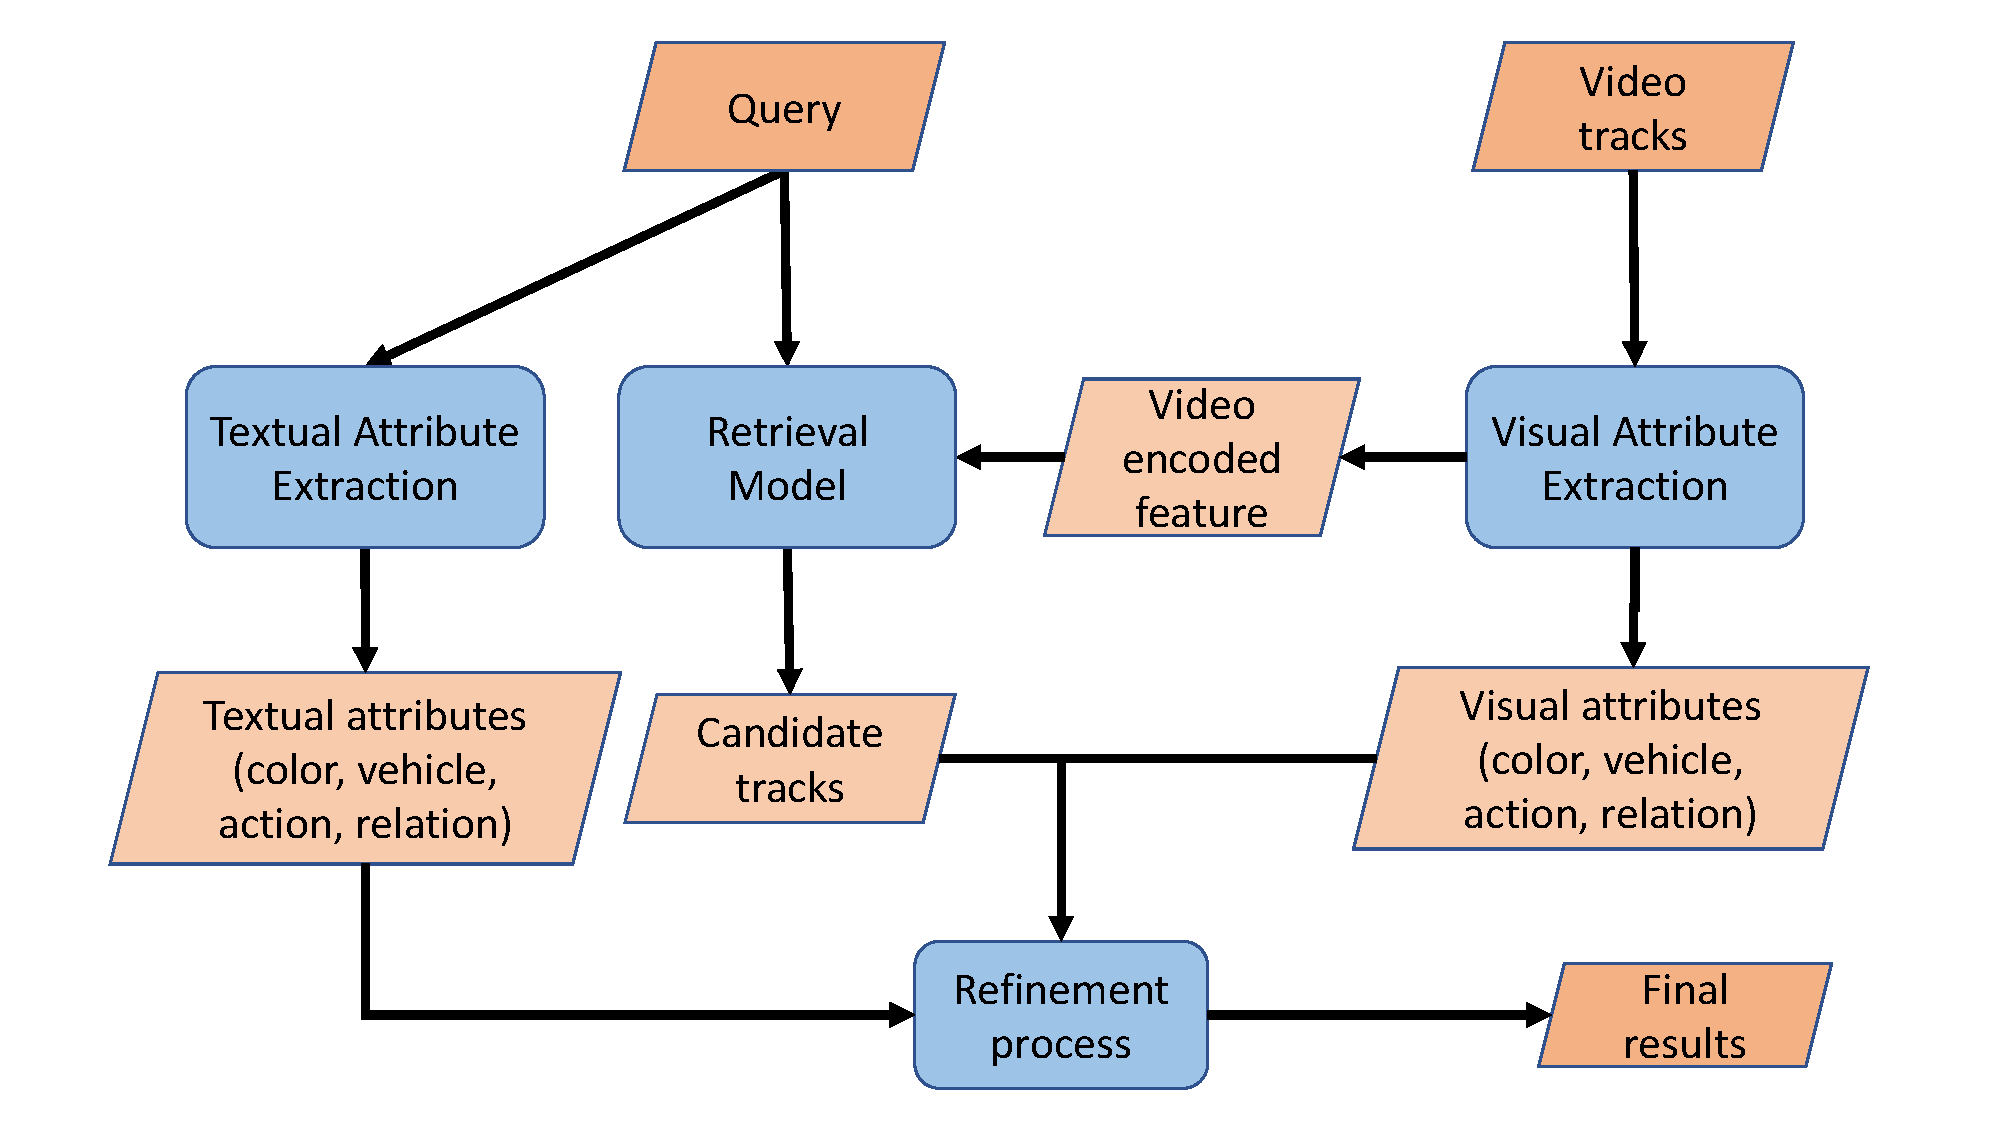
\includegraphics[width=\textwidth]{resources/images/methods/system_overview.pdf}
%     \caption{The overview of our proposed method. The dark orange cells denote the raw inputs and final outputs of the system, while the light ones indicate the intermediate results used in the following stages. The other blue blocks named the four main processing modules: textual/visual attribute extraction, retrieval model, and refinement process.}
%     \label{fig:method_overview}
% \end{figure}

% Our proposed method contains four main parts. With a query and list of video tracks, we first extract essential features in both branches. 
% Given pair of video-text input, Query Analysis and Video Analysis extract appearance attributes, movement behavior and 
% In the first step, not only the textual extraction (module \ref{sec:text_extraction}) aims to localize and obtain the potential attributes of each target vehicle in the given descriptions, but the visual extraction (module \ref{sec:video_extraction}) also provides the same attributes and representation feature based on the vehicle visual context and movement trajectory. 
% Then we utilize a representation learning-based retrieval model \ref{sec:retrieval_model} to produce a list of candidate tracks for each query. 
% The final result is re-ranked by a refinement block \ref{sec:refinement}, using the extracted attributes from previous steps. The overview of our method is explained in Figure \ref{fig:method_overview}.

\begin{figure}[!htb]
    \centering
    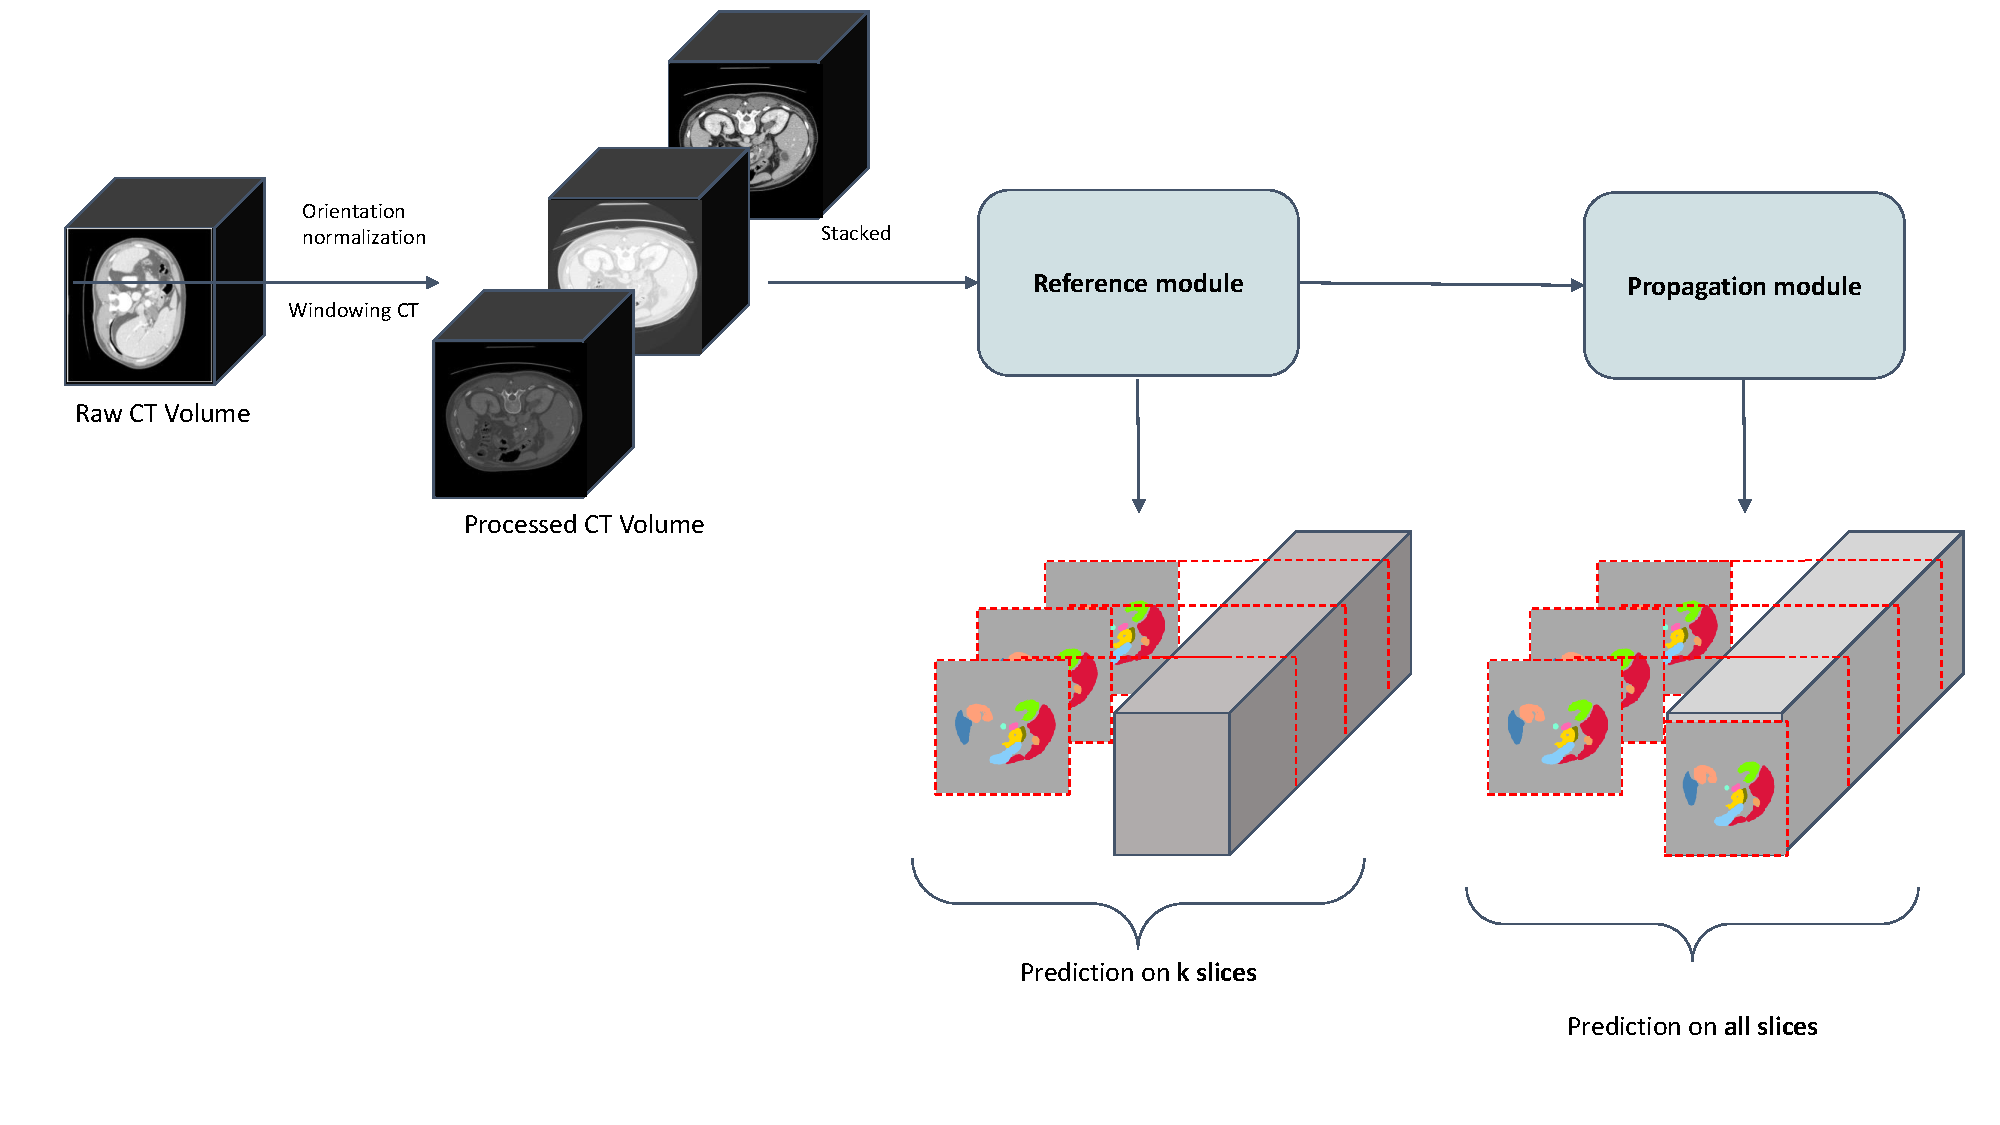
\includegraphics[width=\textwidth]{content/resources/new_images/overview.pdf}
    \caption{The overview description of our proposed pipeline. After the pre-processing stage, a small number of masks are generated across the CT volume by the Reference module. Then these masks are inherited by the Propagation module for the prediction of the remaining slices.}
    \label{fig:method_overview}
\end{figure}

Our proposed method contains two main modules, a reference module and a propagation module.
Firstly, the entire CT volume is processed using windowing CT to get a stack of three-channel slices. \ref{}
Next, a small yet sufficient amount of potential slices are sampled from the stack using a reference strategy to become candidates. These candidate slices progress through the Reference module to obtain the minimal number of preliminary masks.
Afterward, the Propagation module disseminates the information deduced from these initial masks to the remaining slices.
Ultimately, the result is obtained after the final post-processing stage, which includes re-orientation and converting into appropriate format for later usage.

Furthermore, to effectively create pseudo-labels that are consistent for the unlabeled data, we follow the uncertainty estimation technique based on consensus voting scheme. These pseudo-labels that have high certainty level are used for retraining in the next cycle.

The overview of our method is explained in Figure \ref{fig:method_overview}